\documentclass[11pt,a4paper,oneside]{report}

% Encoding & font
\usepackage[T1]{fontenc}
\usepackage[utf8]{inputenc}
\usepackage{lmodern}
\usepackage{microtype}
\frenchspacing
\pdfminorversion=7

\usepackage[british]{babel}

% Page layout
\usepackage[a4paper,left=20mm,right=20mm,top=25mm,bottom=25mm,includefoot]{geometry}
\setlength{\parindent}{0pt}
\setlength{\parskip}{6pt plus 1pt minus 1pt}
\raggedbottom

\usepackage{setspace}
\setstretch{1.05}

% Graphics & floats
\usepackage{graphicx}
\graphicspath{{figures/}{../eda_plots/}}
\usepackage{float}
\usepackage{flafter}
\usepackage{etoolbox}

\makeatletter
\patchcmd{\tableofcontents}{\@starttoc}{\vspace{-1.0cm}\@starttoc}{}{}
\renewcommand*\l@chapter[2]{%
  \ifnum \c@tocdepth >\m@ne
    \addpenalty{-\@highpenalty}%
    \vskip 0.2em \@plus\p@ 
    \setlength\@tempdima{1.5em}%
    \begingroup
      \parindent \z@ \rightskip \@pnumwidth
      \parfillskip -\@pnumwidth
      \leavevmode \bfseries
      \advance\leftskip\@tempdima
      \hskip -\leftskip
      #1\nobreak\hfil \nobreak\hb@xt@\@pnumwidth{\hss #2}\par
      \penalty\@highpenalty
    \endgroup
  \fi}
\makeatother

\usepackage[font=small,labelfont=bf]{caption}
\usepackage{subcaption}

\setlength{\abovecaptionskip}{4pt}
\setlength{\belowcaptionskip}{2pt}
\setlength{\textfloatsep}{8pt plus 2pt minus 2pt}
\setlength{\intextsep}{6pt plus 2pt minus 2pt}

% Listings (example ``source code'' blocks)
\usepackage{xcolor}
\usepackage{listings}
\lstset{
  basicstyle=\ttfamily\small,
  breaklines=true,
  breakatwhitespace=true,
  frame=single,
  framerule=0.4pt,
  columns=fullflexible,
  aboveskip=0.75\baselineskip,
  belowskip=0.75\baselineskip
}
\renewcommand{\lstlistingname}{Listing}

\usepackage{cite}
\usepackage[hyphens]{url}
\def\UrlBreaks{\do\/\do-\do\.}
\usepackage[hidelinks]{hyperref}

% Compact chapter headings (numbered)
\makeatletter
\newcommand{\mainchapter}[1]{%
  \par\vspace*{10pt}%
  \refstepcounter{chapter}%
  \setcounter{section}{0}%
  \addcontentsline{toc}{chapter}{\protect\numberline{\thechapter}#1}%
  {\parindent \z@ \raggedright \normalfont
    \LARGE\bfseries \thechapter. #1\par\nobreak
    \vskip 8pt}%
}
\makeatother

\newcommand{\npar}{\par \vspace{1.2ex plus 0.3ex minus 0.3ex}\noindent}

\begin{document}

% Avoid duplicate PDF page anchors between unnumbered title and front matter
\hypersetup{pageanchor=false}
% Title page — place optional logo at report/figures/KULeuvenLogo.png
\begin{titlepage}
\fontsize{12pt}{14pt}\selectfont

\begin{center}

\IfFileExists{figures/KULeuvenLogo.png}{%
  
\includegraphics[height=1cm]{figures/KULeuvenLogo.png}\\[0.5cm]
}{%
  {\large KU Leuven}\\[0.5cm]
}

Faculty of Economics \& Business\\

\vspace{2.0cm}

\vspace{4.3cm}

\fontsize{17.28pt}{21pt}\selectfont
\textsc{Advanced Analytics}

\fontsize{12pt}{14pt}\selectfont

\vspace{.3cm}
Course report

\vspace{.3cm}
by

\vspace{.4cm}
Pauline \textsc{De Ryck}, Vince \textsc{Coppens}

\vspace{4.3cm}
Professor~\textsc{F. Put}\\

\vspace{1.2cm}
This paper investigates the concept of {\it Edge Computing}, exploring its architecture, relevance, existing standards and open-source implementations, and evaluating its role within modern distributed systems through literature research and practical experimentation.

\vspace{1cm}
Academic year 2025–2026\\
First Master of Business and Information Systems Engineering\\
Catholic University Leuven

\end{center}
\end{titlepage}

\thispagestyle{empty}
\hypersetup{pageanchor=true}

\pagenumbering{roman}
\begingroup
\let\clearpage\relax
\vspace*{-4cm}
\setcounter{tocdepth}{1}
\begin{spacing}{0.9}
\tableofcontents
\end{spacing}
\endgroup
\clearpage

\pagenumbering{arabic}
\vspace*{-1.5cm}

\mainchapter{Introduction}
This report details the implementation and results of the Advanced Analytics in Business course projects. The work covers four primary tasks: customer lifetime value prediction, image-based classification of Lego minifigures, the development of a Retrieval-Augmented Generation (RAG) system for Steam game recommendations, and multilayer network analysis of the Jeffrey Epstein document corpus.

\section{Code availability}
All source code, data preprocessing scripts, and model training notebooks are provided as supplementary materials in this submission. For convenience and version-controlled auditing, the complete repository is also hosted on GitHub at:
\begin{center}
    \url{https://github.com/BigDataNoSleep/AdvancedAnalytics}
\end{center}

\section{Project overview}
The report is structured into four main chapters, each corresponding to one of the primary assignments:
\begin{itemize}
    \item \textbf{Task 1: Customer lifetime value prediction.} This task involves predicting future customer revenue using historical transaction data, employing various exploratory data analysis techniques, feature engineering, and tree-based gradient boosting models.
    \item \textbf{Task 2: Lego minifigure theme classification.} This task focuses on computer vision, comparing MobileNetV2 and EfficientNetV2S backbones to classify images of Lego minifigures into specific themes.
    \item \textbf{Task 3: LLM-based recommender system.} This task presents a hybrid Retrieval-Augmented Generation system for Steam games, combining dense vector search, sparse BM25 retrieval, and a cross-encoder for reranking, with an interactive front-end.
    \item \textbf{Task 4: Epstein corpus network analysis.} This task applies multilayer network analysis to the Jeffrey Epstein document corpus, exploring social co-travel, bipartite person-location relationships, and financial transactions to map institutional and personal influence.
\end{itemize}


\clearpage

\mainchapter{Task 2: Lego Minifigure Theme Classification}

\section{Introduction}

Deep learning has become the default approach for image classification tasks, with convolutional architectures and transfer learning making it feasible to build competitive models on modest datasets without training from scratch.
This assignment applies that toolkit to a dataset of Lego Minifigures scraped from brickset.com. The target is the \texttt{category} attribute, framing the problem as multiclass classification. Given the strong class imbalance, the label space is restricted to the top-$k$ most frequent categories rather than the full set. The pipeline compares several pretrained backbones, fine-tunes the selected one, and documents the architectural trade-offs and regularisation choices used to keep overfitting in check. Model behaviour is then probed with a confusion matrix and Grad-CAM to identify which regions of the image drive predictions, followed by a critical reflection on what the metrics and visualisations actually reveal about the model's reliability.

\section{Data description}
\subsection{Data sources}
The dataset consists of JPG images of individual minifigures. The figures themselves are visually uniform in pose and framing, but the background varies: most are shot on white, some on light brown, and a smaller subset includes a floor as background. When a figure wears a mask or helmet, the underlying head is typically shown as a smaller inset in the upper-right corner of the image.
Metadata is supplied in \texttt{minifigs.json}, with one entry per figure. The fields relevant to this assignment are:
\begin{itemize}
    \item \texttt{category}: heavily imbalanced, ranging from 3,522 objects in the largest class down to a single object in the smallest
    \item \texttt{year\_released}: spans 1975 to 2026
    \item \texttt{current\_value\_used} / \texttt{current\_value\_new}: strings formatted as either "\textasciitilde{}€4.21" or "Not known"
    \item \texttt{themes}: only 87 figures carry three or more theme labels.
\end{itemize}
The remaining fields (\texttt{id}, \texttt{name}, \texttt{link}, \texttt{year}, \texttt{img\_}\allowbreak\texttt{url}, \texttt{minifig\_}\allowbreak\texttt{number}, \texttt{subcategory}, \texttt{set\_}\allowbreak\texttt{id}, \texttt{character\_}\allowbreak\texttt{name}, and \texttt{img\_}\allowbreak\texttt{local\_}\allowbreak\texttt{path}) are not used for the classification task.

\subsection{Data structure}
The JPG files are not stored in the same order as the entries in the JSON file, so the first preprocessing step is to align each image with its corresponding metadata record (via \texttt{minifig\_number} / \texttt{img\_local\_path}) before any splitting or training can take place.

\section{Choice of modelling objective}
Of the three proposed candidate deep learning models, we decided to go forward with Multiclass classification. The multilabel formulation was discarded on the grounds of insufficient signal: only 87 objects carry three or more theme labels, leaving the multilabel structure too sparse to justify the added complexity. Regression was also set aside. Predicting the year of release was deemed too ambiguous to yield reliable visual features, and predicting the value is complicated by its string format. The analysis of this format would preclude the use of GRAD-CAM for visual explainability of the classifications. 

\section{Data preprocessing and assessment of top-$k$ category count and pre-trained backbone}
\subsection{Train/Validate/Test split}
We consecutively applied a stratified 70/15/15 split over the retained top-$k$ categories. Stratification was applied at the category level so that each subset preserves the global class distribution. This matters because the within-top-$k$ distribution is highly imbalanced (e.g. for the top-40 setup, the largest class is 65$\times$ the smallest class), and an unstratified split would magnify that imbalance in evaluation.
For the same reason, macro F1 was chosen as the evaluation metric. It averages F1 across classes with equal weight, so performance on small categories counts as much as performance on large ones. Plain accuracy would be dominated by the largest classes and would mask failures on the long tail.

\subsection{Top-$k$ category count}
The first two runs both used \texttt{MobileNetV2} as backbone from \texttt{keras.applications}, with a frozen ImageNet-pretrained backbone, balanced class weights, and an otherwise identical training procedure. The only variable was the label space: top-64 versus top-20. Macro F1 came in at 0.57 and 0.68 respectively, a gap of 0.11. Because architecture and training procedure were held constant, this gap is attributable cleanly to category count.
To balance informativeness against per-class sample size, $k=40$ was chosen for the main model. This retains 33\% of the original 122 categories while still implying a 65$\times$ imbalance between largest and smallest class (3,522-54 samples).
A possible alternative was to keep the top 40 and bin the remaining 82 categories into a single "Other" class. This was rejected: with more than two thirds of categories collapsed into one bucket, "Other" would dominate the loss and distort the macro F1, while training pressure would be diverted away from the categories that actually matter.

\subsection{Pre-trained backbone}
Backbones were compared on the top-20 setup rather than top-40, reusing the \texttt{MobileNetV2} run from 4.2 as the baseline. The run was compared to \texttt{EfficientNetV2S}, a heavier, more recent backbone demanding a higher resolution (384$\times$384 versus 224$\times$224 for \texttt{MobileNetV2}), also from \texttt{keras.applications}. Macro F1 moved from 0.68 to 0.70. The improvement is real but smaller than the top-$k$ gap, and since category count is held constant, the 0.02 reflects architecture alone: \texttt{EfficientNetV2S} extracts somewhat stronger features from this dataset.
\texttt{EfficientNetV2S} was selected for the main model. The comparison was run with a frozen base, so the 0.02 gain measures only the quality of the pretrained features feeding into the head. With partial fine-tuning of the upper layers (Section 6), the stronger backbone has more room to adapt and the gap is expected to widen.

\section{Data and preprocessing}
\subsection{Splits and resolution}
As mentioned before, we applied a stratified 70/15/15 split over the 40 retained categories. Images were loaded at 384$\times$384 through Keras's \texttt{ImageDataGenerator} with batch size 16.
No custom preprocessing of backgrounds or minifig framing was applied. Although backgrounds occasionally deviate from the standard white (light brown, floor scenes), the minifigures themselves are near-uniform in size and position within the frame, so a generic crop or background-removal pass risked introducing more noise than it removed. This decision was validated post-hoc via Grad-CAM (Section 8.2): the activation maps consistently focus on the minifigure body rather than the background, and for figures with an inset head in the upper-right corner, on the main figure rather than the inset.
The \texttt{rescale} parameter of \texttt{ImageDataGenerator} was deliberately left at \texttt{None} as \texttt{EfficientNetV2} includes a built-in normalisation layer.

\subsection{Augmentation}
Augmentation was applied to the training generator only, leaving the validation and test generators (\texttt{shuffle=False} on the latter) untouched so that evaluation runs on unaltered images. The training pipeline applied random rotations of up to 30$^\circ$, horizontal and vertical shifts of up to 20\%, brightness scaling in the [0.8, 1.2] range, horizontal flipping, and zooming up to 20\%, with nearest fill for any newly exposed pixels.

\subsection{Initial class weights}
To handle category imbalance, we computed balanced weights using the \texttt{compute\_}\allowbreak\texttt{class\_}\allowbreak\texttt{weight} function (with \texttt{class\_}\allowbreak\texttt{weight='balanced'}) from \texttt{sklearn}. Since macro F1 is our headline metric and weighs every class equally regardless of support, the loss function needs to treat them equally too. Without weighting, the optimiser would minimise loss most effectively by getting frequent classes right and effectively ignoring the rare ones. These weights were passed through the \texttt{class\_weight} argument of \texttt{model.fit} and applied in both Phase 1 and Phase 2. We return to them in Section 7.

\section{Model and two-phase training}
\subsection{Architecture}
The model uses \texttt{EfficientNetV2S} as the feature extractor, initialised with ImageNet weights. On top of the convolutional base we built a custom head as a \texttt{Sequential} stack: \texttt{GlobalAveragePooling2D} to collapse the spatial dimensions, then a \texttt{BatchNormalization} layer, a \texttt{Dense(512, relu)} for the task-specific projection, a \texttt{Dropout(0.4)} for regularisation, a second \texttt{BatchNormalization}, and a final \texttt{Dense(40, softmax)} for the multiclass output.

\subsection{Phase 1: head training}
In the first phase the entire \texttt{EfficientNetV2S} backbone was frozen (\texttt{base\_model.trainable = False}), so gradients flowed only into the new head. The model was compiled with the Adam optimizer at a learning rate of $10^{-3}$, a deliberately high starting point, since at this stage we are training only freshly initialised dense weights. The loss function was \texttt{categorical\_crossentropy} against the one-hot targets, and we tracked accuracy, Precision, and Recall alongside loss, relevant given the macro-F1 framing.

\subsection{Phase 2: partial fine-tuning}
The base model was unfrozen, after which we re-froze all but the last 100 layers, roughly the top fifth of \texttt{EfficientNetV2S}, which has 513 layers in total. The reasoning is standard transfer-learning logic: lower layers encode generic visual primitives (edges, textures, colour gradients) that ImageNet already learned well on a far larger dataset than ours, while upper layers encode dataset-specific abstractions that benefit from adaptation to Lego minifigures.
The model was recompiled with a learning rate of $10^{-5}$, two orders of magnitude below Phase 1. This is essential to avoid catastrophic forgetting, where large weight updates erase the useful pretrained features we are trying to preserve. The loss function, metrics and class weights were unchanged. 

\section{Initial evaluation and class-weight smoothing}
\subsection{Initial evaluation}
After the two-phase training, the model was evaluated on the held-out test set. Overall accuracy reached 60\%, with a macro F1 of 0.58, macro precision of 0.54, and macro recall of 0.73. Macro F1 is the metric we focus on: by weighting every class equally regardless of support, it ensures that strong performance on rare categories is not buried under the bulk of frequent ones.
The precision-recall gap is the most informative number here. Recall at 0.73 means the model successfully retrieves most relevant instances across classes, but precision at 0.54 means more than four in ten of its positive predictions are wrong. The pattern was concentrated in the smaller classes, where recall was often near-perfect and precision floored out, a signature of a classifier that has been pushed too hard toward minority classes.

\subsection{Square-root smoothing}
The cause traces back to the standard \texttt{class\_weight='balanced'} setting from Section 5.3, which assigns each class a weight inversely proportional to its frequency. For a top-40 distribution where the rarest class has 65$\times$ fewer samples than the most frequent, this produces extreme weight ratios. The optimiser responds rationally: it lowers the decision threshold for rare classes, accepting a flood of false positives in exchange for catching every true case.
The fix is to compress the weight range without changing its rank order. We applied a square-root transformation to the balanced weights, \texttt{np.sqrt(balanced\_weights)}, which preserves the principle that rare classes deserve more weight than frequent ones but pulls the most extreme weights toward the median. 
The best-validation-loss checkpoint from the two-phase run was then reloaded and the model recompiled with the smoothed weights at a learning rate of $10^{-6}$: one order of magnitude below Phase 2, since the goal is now a gentle re-balancing of an already fine-tuned model rather than further feature adaptation.

\subsection{Final evaluation}
Re-evaluating on the held-out test set after the smoothed-weight pass produced 62\% accuracy, with a macro F1 of 0.60, macro precision of 0.56, and macro recall of 0.73. Accuracy moved up two points, macro F1 gained 0.02, precision rose by 0.02, and recall held flat.
The recall stability is the most important read on these numbers. Compressing the weight range reduces the optimiser's incentive to overpredict rare classes, which would normally come at the cost of recall as the model becomes more conservative, but recall did not move. The precision gain therefore came from genuinely cleaner decisions rather than from trading away coverage. The F1 improvement is modest in absolute terms but consistent with the diagnosis in 7.1: the original problem was a precision deficit on rare classes, and that is precisely where the smoothing acted.

\section{Visual analysis}
\subsection{Confusion patterns}
To establish where the model goes wrong before asking why, we plot the test-set predictions as a 40$\times$40 confusion matrix (Figure \ref{fig:confusion_matrix}). The diagonal is strongest for the four largest classes (DUPLO, Town, Friends, and Star Wars) which is expected: more training data buys cleaner decision boundaries. 
The clearest structural pattern off the diagonal is the Town row, which spreads thinly across many columns: when a true Town minifigure is misclassified, it scatters across a wide range of themes rather than concentrating on any single confuser. This matches what Town actually is, a category of generic civilian minifigures without distinctive theme decals and the symmetric scatter into the Town column from other rows suggests it also functions as the model's default guess when no theme-specific cues are present. Beyond Town, off-diagonal mass concentrates around visually similar movie and franchise themes (Star Wars, Super Heroes, The LEGO NINJAGO Movie), where the figures genuinely share design language and additional training data on its own would not resolve the ambiguity. 

\begin{figure}[H]
    \centering
    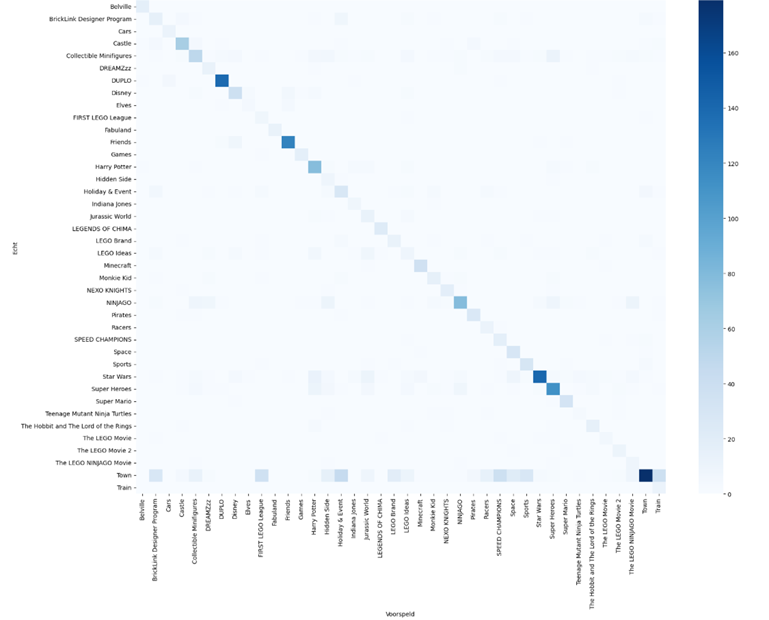
\includegraphics[width=\textwidth]{figures/A2_confusion_matrix.png}
    \caption{Confusion matrix for the top-40 Lego minifigure theme classification task.}
    \label{fig:confusion_matrix}
\end{figure}

\subsection{Grad-CAM}
\subsubsection{Set up}
The confusion matrix tells us which classes the model confuses; it does not tell us why. To inspect which regions of the image actually drive each prediction, we implemented Grad-CAM on the last convolutional layer of the \texttt{EfficientNetV2S} backbone (\texttt{top\_activation}). The procedure follows the standard formulation: we compute the gradient of the predicted class score with respect to the feature maps of that layer, pool those gradients spatially to obtain per-channel importance weights, and take a weighted sum of the feature maps using those weights. A ReLU and per-image normalisation produce a heatmap in [0, 1] indicating where attention concentrated for the chosen prediction.
For visualisation, we applied a 60th-percentile threshold to the heatmap to suppress low-attention regions before colouring, used the \texttt{inferno} colormap on the surviving values, and blended the result into the original image at a 0.55 / 0.7 ratio (heatmap / image). We ran the visualiser on 10 random test images, with each row showing the original, the overlay, and a summary block stating the predicted class, confidence, and whether the prediction was correct.

\subsubsection{Observations}
For correctly classified high-confidence cases, attention concentrates tightly on class-distinctive decals. On the Star Wars Darth Vader figure (97.5\% confidence) the heatmap locks onto the chest control panel and helmet. On the DUPLO firefighter (99.5\%) attention is on the helmet badge and the torso radio, both characteristic DUPLO printed elements. These are the cases the macro-F1 number is built on: the model has learned the right cues for the well-represented themes.
The more informative cases sit at the lower-confidence end. The Town civilian, correctly classified at 48.2\%, shows diffuse attention spread across the head and shoulders without any single cue dominating, consistent with a figure that simply carries no theme-specific decals to anchor on. A similar pattern appears for the Super Heroes Hulk (48.5\%), where diffuse torso attention reflects the fact that the Hulk's oversized non-standard proportions sit far outside the Super Heroes figures the model trained on. The confidence calibration is doing useful work here: low-confidence correct predictions correspond to genuinely ambiguous inputs, not random underconfidence.
The misclassification example illustrates the limit of what additional training can fix. A NINJAGO figure was predicted as Monkie Kid at 86.9\% confidence, with the heatmap focused on its head. The attention is on the right region but draws the wrong conclusion, because that visual signature exists in both themes. The model is reading the image correctly; the label boundary is what's underdefined. The off-diagonal bleed between visually similar themes in the confusion matrix reflects the same underlying problem.

\begin{figure}[H]
    \centering
    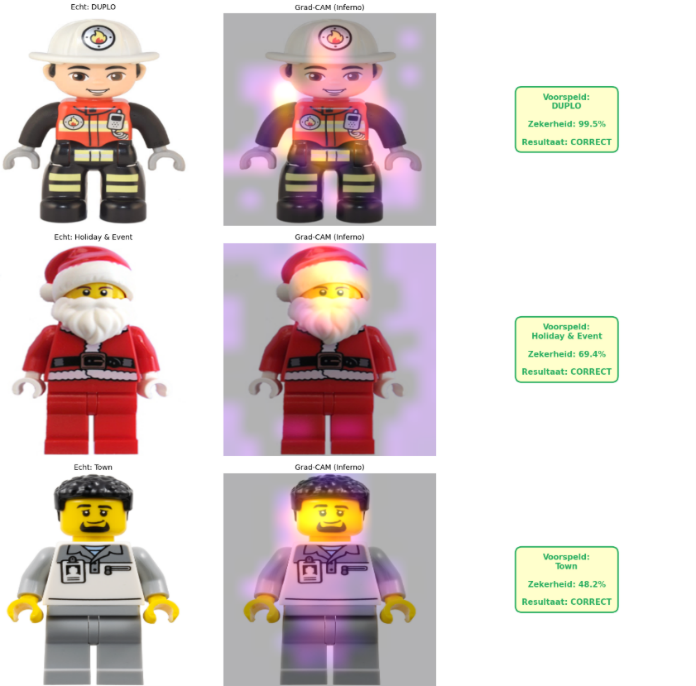
\includegraphics[width=0.85\textwidth]{figures/A2_GRADCAM1.png}
    \caption{Grad-CAM: High-confidence correct classification (Star Wars Darth Vader).}
\end{figure}

\begin{figure}[H]
    \centering
    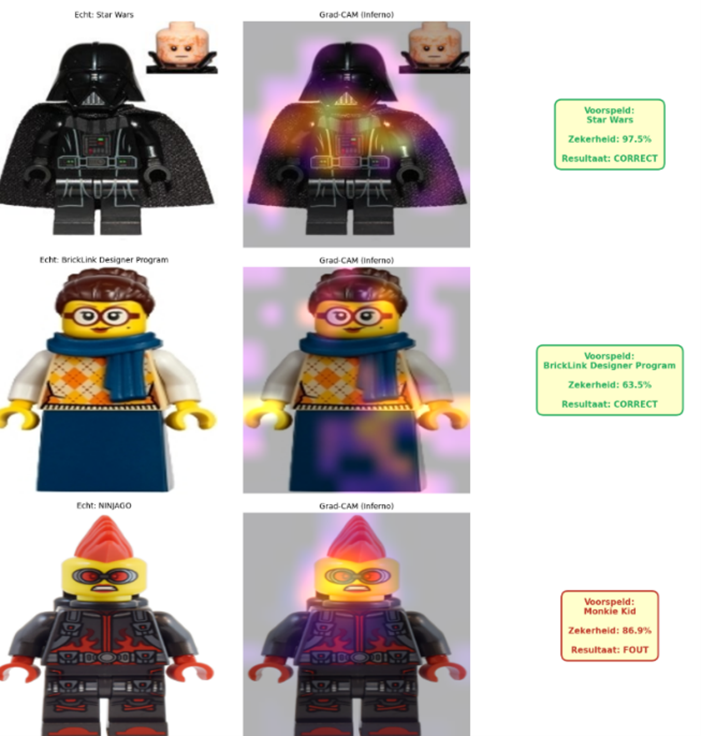
\includegraphics[width=0.85\textwidth]{figures/A2_GRADCAM2.png}
    \caption{Grad-CAM: Low-confidence correct prediction (Town civilian).}
\end{figure}

\begin{figure}[H]
    \centering
    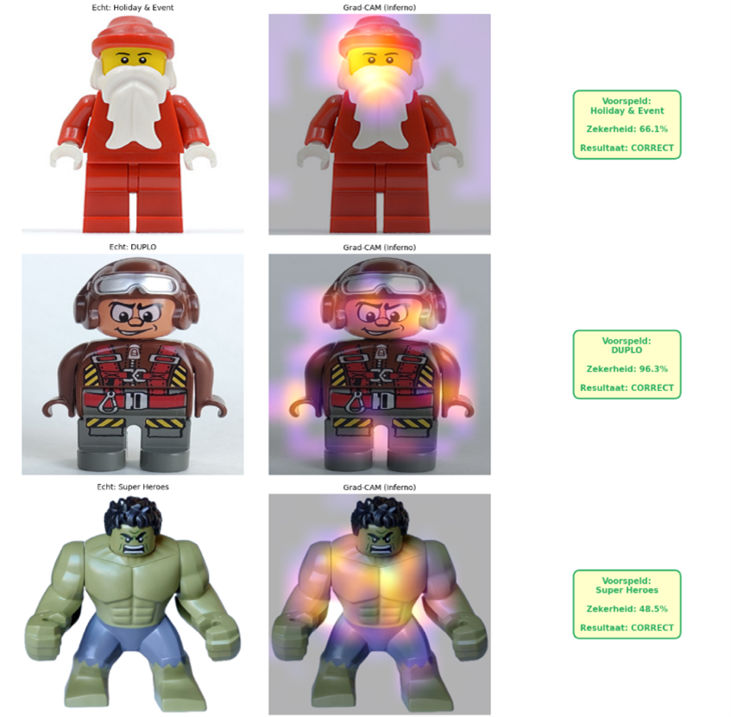
\includegraphics[width=0.85\textwidth]{figures/A2_GRADCAM3.png}
    \caption{Grad-CAM: Misclassification due to visual similarity (NINJAGO vs Monkie Kid).}
    \label{fig:gradcam}
\end{figure}

\section{Conclusion}
We arrived at a final macro F1 of 0.60 (62\% accuracy) on the top-40 test set, using \texttt{EfficientNetV2S} with a partially fine-tuned backbone, a custom head, and square-root-smoothed class weights. The three preliminary runs in Section 4 framed this as a defensible operating point: trimming the long tail did most of the heavy lifting on macro F1, while the backbone upgrade contributed a smaller but real margin on top. $k=40$ captures most of the category-count gain without trimming so aggressively that the task loses breadth, and \texttt{EfficientNetV2S} was retained on the expectation, borne out by the final result, that fine-tuning would extend its frozen-base advantage.
The biggest single in-training contributor was the class-weight smoothing in Section 7.2. The standard \texttt{class\_weight='balanced'} setting, which we initially treated as a sensible default, was in fact actively distorting the optimisation by depressing precision on rare classes. Reducing the weight range with a square-root transform, then applying a brief 3-epoch correction at a $10^{-6}$ learning rate, recovered roughly two points of macro F1 without forfeiting recall. Diagnostic refinement of an existing default outperformed any further architectural change we could plausibly have made within the time available, a useful lesson in where the marginal returns actually sit.
We also believe that further gains from this point are unlikely to be cheap. The remaining error mass concentrates in two places, both visible in Section 8: classes with limited training data and no distinctive visual cues (Town being the clearest case, where Grad-CAM showed diffuse attention because there is no theme-specific decal to anchor on), and clusters of themes that share design language so closely that the model attends to the right region but draws the wrong conclusion (the NINJAGO--Monkie Kid case being typical). Neither problem yields to backbone choice or hyperparameter sweeps. More data per rare class would help directly with the first, but is outside the scope of the assignment. A hierarchical approach, predicting a coarse theme cluster first, then a subtheme conditional on that, might reduce the precision penalty on the second, since classification within a cluster could focus on discriminating features rather than competing against 39 unrelated alternatives. Either of these would be a substantive next step rather than a tuning exercise, and we judge that the current result is a reasonable place to stop.


\clearpage

\mainchapter{Task 3: LLM-Based Recommender System}

\section{Introduction}
This project aims to develop an LLM-based recommender system for Steam games that can interpret natural language queries and generate meaningful recommendations. Unlike traditional systems that rely heavily on exact keyword matching or user-item interaction matrices, this system focuses on understanding the intent behind user queries.

The implemented solution follows a Retrieval-Augmented Generation (RAG) approach, combining structured retrieval with generative modeling to ensure factual and flexible recommendations. This architectural pipeline begins with an initial self-querying step using \texttt{Gemma 3 12B IT}, which serves as both a query optimizer and a robust guardrail for relevance. The retrieval mechanism then employs a hybrid strategy, merging semantic search capabilities with keyword-based search via BM25 to capture both user intent and exact matches. Finally, the system leverages the Gemma model through the Gemini API to refine candidate games and generate grounded, human-like recommendations based on the retrieved context.


\section{Dataset and Preprocessing}
The dataset is stored in a SQLite database (\texttt{steam\_games\_reviews\_25.sqlite}) containing Steam data scraped up to April 2026. It consists of two tables: \texttt{games} and \texttt{reviews}.

The \texttt{games} table includes metadata such as game name, description, genres, tags, price, release date, platform compatibility, and review statistics. The \texttt{reviews} table contains user-generated reviews linked via the game’s application ID, including the review text, language, and a \texttt{weighted\_vote\_score} indicating helpfulness.

To ensure manageable performance, the system indexes up to 5,000 games. Although each game may contain up to 500 English reviews, only the top three reviews per game are used during recommendation. These are selected based on their helpfulness score to ensure that the most informative feedback is prioritised.

Preprocessing was necessary to standardise the data. Tags were extracted from potentially nested structures and reduced to the top eight to prevent excessive noise. Additionally, a combined textual representation was constructed for each game, merging name, genres, tags, and description into a single structured document. Explicit prefixes were added to guide downstream models.

\section{System Architecture}
The system is built as a multi-stage pipeline consisting of query optimisation, hybrid retrieval, re-ranking, and final generation. This design was chosen to maximise both relevance and interpretability.

\begin{figure}[!t]
    \centering
    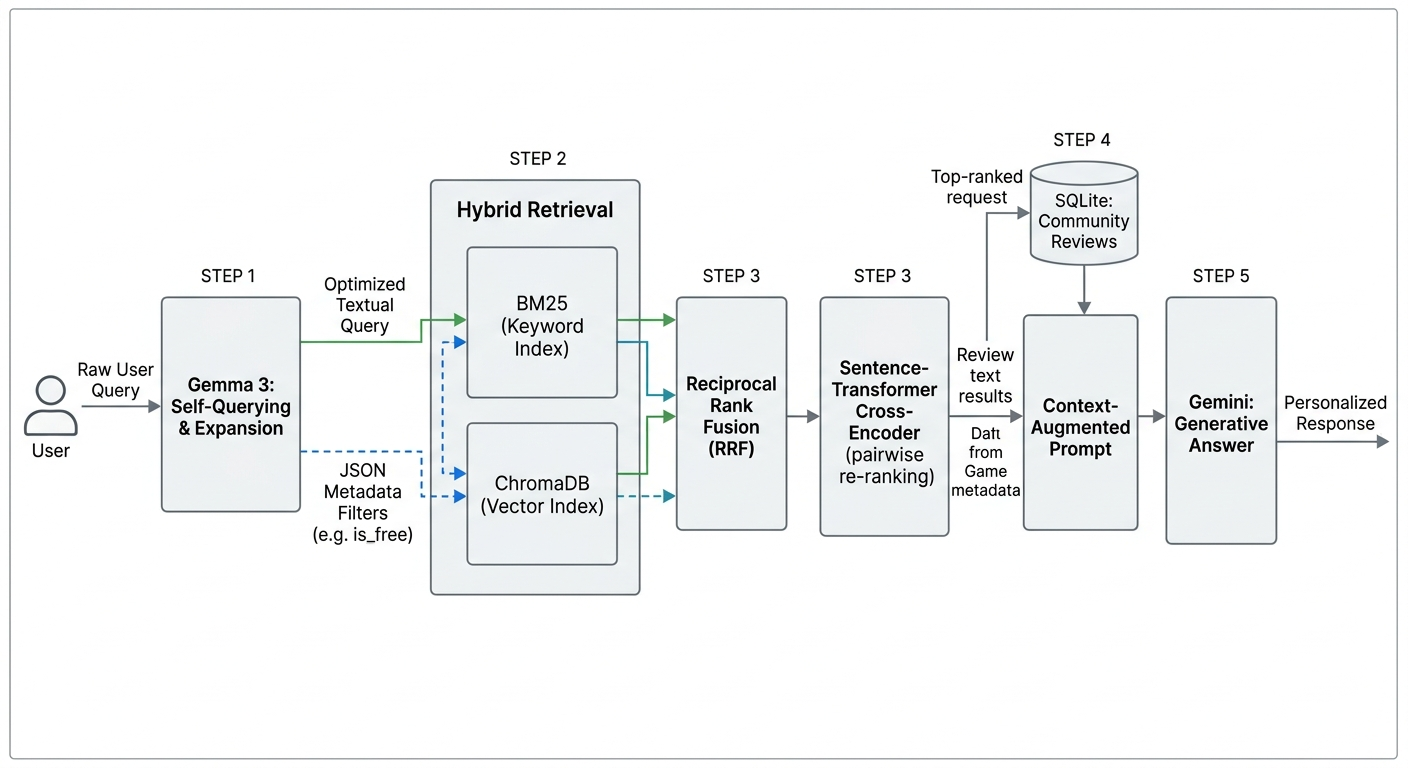
\includegraphics[width=\textwidth]{figures/3_1.png}
    \caption{System Architecture of the RAG-based Steam Recommender System.}
    \label{fig:architecture}
\end{figure}

A key component is the initial self-querying step using \texttt{Gemma 3 12B IT}. The user’s raw query is first rewritten into a more structured and optimised search query. At the same time, the model extracts explicit constraints such as price requirements. For instance, a query requesting ``free games'' is converted into a structured filter that can be applied during retrieval. This step also serves as a guardrail. If the query is unrelated to games, the system returns a \texttt{NOT\_RELEVANT} signal and bypasses the recommendation pipeline entirely.

The backend is implemented in Flask, with indexing performed in a background thread. Additionally, Server-Sent Events (SSE) are used to stream intermediate pipeline information to the frontend, improving transparency and debuggability.

\section{Retrieval, Ranking and Embedding Strategy}
The retrieval stage combines semantic and keyword-based methods. Semantic search is implemented using ChromaDB, which stores vector embeddings of game documents. Keyword search is performed using BM25, which captures exact term matches.

Each method retrieves 30 candidates, which are then merged using Reciprocal Rank Fusion. This approach ensures that both semantic similarity and exact keyword relevance contribute to the final candidate set. Filters extracted during the self-querying stage are applied at this point.

An important design decision concerns the embedding model. Initially, the system was intended to use Google’s Gemini embedding model (\texttt{gemini-embedding-2}) to achieve higher semantic quality. However, during implementation, this approach proved impractical due to strict rate limits in the free API tier. Embedding thousands of games resulted in frequent failures and long runtimes.

As a result, the system was adapted to use the local Sentence Transformers model \texttt{all-MiniLM-L6-v2}. While smaller, this model runs entirely locally and enables fast, stable indexing. Embeddings are stored persistently in ChromaDB with cosine similarity, and batch insertion is used to improve robustness.

After retrieval, candidates are re-ranked using a cross-encoder model (\texttt{ms-marco-MiniLM-L-6-v2}). This model evaluates query–game pairs directly, producing more accurate relevance scores than embedding-based methods alone. The top five results are selected for generation, with an additional heuristic to exclude games explicitly mentioned in the query.

\section{Generation and Use of Reviews}
The final recommendation is generated using the Gemma model via the Gemini API. The prompt includes detailed information for each selected game, such as ranking position, price, release date, tags, review statistics, and a short description.

A crucial component of this stage is the integration of player reviews. For each candidate game, the system performs a real-time SQLite query to retrieve the most relevant reviews:

\begin{lstlisting}[language=SQL, caption=SQL query for fetching top helpful reviews.]
SELECT review FROM reviews 
WHERE appid = ? AND language = 'english' 
ORDER BY weighted_vote_score DESC 
LIMIT 3;
\end{lstlisting}

Rather than performing an additional semantic search over the review corpus, which would introduce significant computational overhead, the system relies on Steam’s built-in community ranking mechanism. Reviews are selected strictly based on their \texttt{weighted\_vote\_score}, which reflects how many users found a review helpful, adjusted through Steam’s internal weighting. By filtering for English-language reviews and selecting only the top-ranked entries, the system effectively uses community consensus as a quality signal.

The impact on recommendation quality is significant. The LLM is explicitly instructed to reference these reviews when generating its response, forcing it to justify recommendations using real player feedback. This enables the system to capture nuances---such as difficulty level, social aspects, or recurring criticisms---that are often absent from developer-written descriptions. Consequently, the generated recommendations are more grounded, balanced, and trustworthy.

\section{Evaluation, Challenges and Future Work}
The system was evaluated through manual testing across a variety of query types, including genre-specific requests, constraint-based queries, and irrelevant inputs. The integration of review data was particularly effective in improving realism.

However, the system introduces noticeable latency due to its multi-stage design. Each query involves multiple steps, including two LLM calls and cross-encoder inference, which increases response time.

Additional challenges included handling inconsistent LLM outputs (such as JSON formatting issues) and ensuring compatibility between metadata and database queries. The dataset size is also limited, which restricts the system’s ability to recommend very niche titles.

\section{Conclusion}
This project demonstrates how LLMs can be effectively integrated into recommender systems using a Retrieval-Augmented Generation framework. By combining hybrid retrieval, cross-encoder re-ranking, and grounded generation, the system is able to produce accurate and context-aware recommendations.

A key insight is that combining semantic and keyword-based retrieval leads to more robust results than relying on a single method. Additionally, incorporating player reviews significantly improves the credibility of the recommendations.

\section{Running the Project}
To ensure that the project can be evaluated without friction, the system has been designed for straightforward setup and execution. The only requirement is a machine running Python 3.10 or higher. As mentioned in the introduction of this report, the complete source code for this system is provided as a supplementary file in the submission and is also publicly available on GitHub for version-controlled auditing.

Dependencies can be installed using \texttt{uv}, which is recommended for speed and reliability:

\begin{lstlisting}[language=bash]
cd raglooker
uv sync
\end{lstlisting}

Alternatively, the required packages can be installed with \texttt{pip}:

\begin{lstlisting}[language=bash]
pip install flask ollama rank-bm25 chromadb sentence-transformers google-genai python-dotenv matplotlib scikit-learn numpy
\end{lstlisting}

The application can then be launched with:

\begin{lstlisting}[language=bash]
uv run app.py
\end{lstlisting}

On first startup, a background daemon thread initialises both the ChromaDB vector database and the BM25 index. The application can then be accessed via the local address shown in the terminal (typically \texttt{http://127.0.0.1:5000}).

\section{Implementation Details}
For a deeper technical dive into the core algorithms described in this chapter, including the self-querying expansion logic, the hybrid Reciprocal Rank Fusion retrieval, and the cross-encoder re-ranking implementation, please refer to the code snippets provided in \textbf{Appendix A}.


\clearpage


%\clearpage

\mainchapter{Appendix}
\section*{Appendix A: Technical Implementation of Task 3}
\addcontentsline{toc}{section}{Appendix A: Technical Implementation of Task 3}

This appendix contains the primary implementation logic for the Steam RAG Recommender system, with key segments extracted from the \texttt{recommender.py} file.

\subsection*{A.1 LLM-Based Query Expansion and Guardrails}
The system uses \texttt{Gemma 3 12B IT} to perform self-querying. This stage optimizes the user's natural language input for vector search while extracting metadata constraints and enforcing a relevance guardrail.

\begin{lstlisting}[language=python, caption=The query expansion and guardrail implementation.]
def rewrite_query(self, query: str) -> dict[str, Any]:
    prompt = (
        f"You are a search query guardrail and expansion expert for a Steam game recommendation engine.\n"
        f"A user entered the following search query: \"{query}\"\n\n"
        f"Please rewrite and expand this query to be optimal for vector similarity search against a database of game descriptions and tags.\n"
        f"Include relevant genres, sub-genres, gameplay mechanics, and thematic keywords.\n"
        f"RULES:\n"
        f"1. If the query is about video games, expand it for vector similarity search.\n"
        f"2. If the query is unrelated (e.g., cooking recipes), output ONLY 'NOT_RELEVANT'.\n"
        f"3. You must respond with ONLY valid JSON in the following format:\n"
        f"{{\n"
        f"  \"search_string\": \"keywords, genres, themes...\",\n"
        f"  \"filters\": {{\"is_free\": true_or_false}}\n"
        f"}}\n"
    )
    try:
        response = self.client.models.generate_content(model=LLM_MODEL, contents=prompt)
        text = response.text.strip()
        if "NOT_RELEVANT" in text.upper() and not text.startswith("{"):
            return {"search_string": "NOT_RELEVANT", "filters": {}}
        
        # Cleanup markdown formatting if present
        if text.startswith("```json"): text = text[7:-3].strip()
        return json.loads(text)
    except Exception as e:
        return {"search_string": query, "filters": {}}
\end{lstlisting}

\subsection*{A.2 Hybrid Retrieval and Reciprocal Rank Fusion (RRF)}
The retrieval engine combines semantic embeddings and exact keyword matching.

\begin{lstlisting}[language=python, caption=The Hybrid Search and RRF merging logic.]
def retrieve_candidates(self, query: str, filters: dict[str, Any]) -> list[GameRecord]:
    n_retrieve = 30
    
    # 1. Metadata Filtering for ChromaDB
    where_clause = {"price": 0.0} if filters.get("is_free") else None

    # 2. Vector Search (ChromaDB)
    chroma_results = self.collection.query(
        query_texts=[query], n_results=n_retrieve, where=where_clause
    )
    chroma_ids = chroma_results['ids'][0] if chroma_results['ids'] else []

    # 3. Keyword Search (BM25)
    tokenized_query = query.lower().split(" ")
    bm25_scores = self.bm25.get_scores(tokenized_query)
    bm25_ranked = sorted(zip(self.records, bm25_scores), key=lambda x: x[1], reverse=True)
    
    # Apply filters to BM25 results
    if filters.get("is_free"):
        bm25_ranked = [(r, s) for r, s in bm25_ranked if r.raw.get("price", 1.0) == 0.0]
    bm25_ids = [r.app_id for r, _ in bm25_ranked[:n_retrieve]]

    # 4. Combine with Reciprocal Rank Fusion (RRF)
    k = 60
    rrf_scores: dict[str, float] = {}
    for rank, app_id in enumerate(chroma_ids):
        rrf_scores[app_id] = rrf_scores.get(app_id, 0.0) + 1.0 / (k + rank + 1)
    for rank, app_id in enumerate(bm25_ids):
        rrf_scores[app_id] = rrf_scores.get(app_id, 0.0) + 1.0 / (k + rank + 1)

    sorted_app_ids = sorted(rrf_scores.keys(), key=lambda x: rrf_scores[x], reverse=True)
    return [r for r in self.records if r.app_id in sorted_app_ids[:n_retrieve]]
\end{lstlisting}

\subsection*{A.3 Cross-Encoder Re-ranking}
This stage improves precision by performing a full attention pass over the query and candidates.

\begin{lstlisting}[language=python, caption=Cross-Encoder re-ranking implementation.]
def rank_candidates(self, query: str, candidates: list[GameRecord]) -> list[tuple[GameRecord, float]]:
    if not candidates: return []
    pairs = []
    for r in candidates:
        tags = ", ".join(r.raw.get("tags", {}).keys()) if isinstance(r.raw.get("tags"), dict) else ""
        doc = f"Name: {r.name}\nGenres: {', '.join(r.raw.get('genres', []))}\nTags: {tags}\nDescription: {r.short_description}"
        pairs.append((query, doc))
    
    scores = self.cross_encoder.predict(pairs)
    ranked = sorted(zip(candidates, scores), key=lambda x: x[1], reverse=True)
    return [(record, float(score)) for record, score in ranked]
\end{lstlisting}

\subsection*{A.4 Generative Answer with SQL Review Augmentation}
The final stage fetches the most helpful community reviews in real-time to ground the recommendation.

\begin{lstlisting}[language=python, caption=The final generative stage with review injection.]
def _get_top_reviews(self, app_id: str, limit: int = 3) -> list[str]:
    with sqlite3.connect(self.db_path) as conn:
        conn.row_factory = sqlite3.Row
        query = "SELECT review FROM reviews WHERE appid = ? AND language = 'english' ORDER BY weighted_vote_score DESC LIMIT ?"
        rows = conn.execute(query, (app_id, limit)).fetchall()
        return [row["review"] for row in rows if row["review"]]

def generate_answer(self, query: str, matches: list[tuple[GameRecord, float]]) -> str:
    context_items = []
    for i, (record, score) in enumerate(matches):
        reviews = self._get_top_reviews(record.app_id)
        review_text = "\n".join([f"- {rev[:200]}..." for rev in reviews])
        item = (
            f"Rank #{i+1} | Game: {record.name}\n"
            f"Reception: {record.raw.get('positive')} Positive reviews\n"
            f"Player Feedback:\n{review_text}"
        )
        context_items.append(item)

    prompt = (
        f"You are a Steam game recommendation expert. User query: \"{query}\"\n\n"
        f"--- CONTEXT ---\n{chr(10).join(context_items)}\n---------------\n\n"
        f"Rules: Respect ranking order. Use player reviews to justify the recommendation."
    )
    response = self.client.models.generate_content(model=LLM_MODEL, contents=prompt)
    return response.text
\end{lstlisting}


\clearpage

%\addcontentsline{toc}{chapter}{Bibliography}
%
%\bibliographystyle{ieeetr}
%\bibliography{references}



\end{document}
